\cleardoublepage
\chapter{Developed Architectures}

%%%%%%%%%%%%%%%%%%%%%%%%%%%%%%%%%%%%%%%%%%%%%%%%%%%%%%%%%%%%%%%%%%%%%%%%%%%%%%
\section{Software Implementations}

The previous chapter presented some characteristics of the current state of \emph{libaom}'s \emph{Transform} stage which might compromise its performance, the most relevant being the unnecessary flexibility in the representation of cosine approximations.

In order to undertake these opportunities, and improve the overall encoder performance, new architectures for the studied stage were developed. The first approach was to study possible simplifications of the reference software, through the development and testing of alternative approaches for the provided functions.

The developed implementations tackled the forward \emph{DCT}, as it was the \emph{kernel} that would have the most impact on encoder performance. As the \emph{IDCT} is shared between encoder and decoder, and due to the added complexity, no changes were done to this block, as it acts with accordance with the established standard, as mentioned previously. 

All the developed architectures and corresponding tests were written in $C$ programming language, as to maintain the simple integration into \emph{libaom}.

%%%%%%%%%%%%%%%%%%%%%%%%%%%%%%%%%%%%%%%
\subsection{Matrix Multiplication Implementation}

The first test was the application of the simplest integer \emph{DCT}, done by the multiplication of the input vector by a scaled up version of the transform matrix, $\mathbf{F}$, firstly shown in Equation \ref{eq:DCT2}. 

The original integer transform matrix is shown in Equation \ref{eq:matscale}.

\begin{equation} \label{eq:matscale}
    \begin{gathered}
        \mathbf{F}_{x,u} = \beta(u)\cos\left(\frac{(2x+1)u\pi }{2L}\right),\;0\leq u,x < L \\
        \Downarrow \\
        \mathbf{F} = \sqrt{\frac{2}{L}}  \begin{bmatrix}
            \sqrt{\frac{1}{2}}                                  & \sqrt{\frac{1}{2}}                                & \dots & \sqrt{\frac{1}{2}} \\
            \cos\left(\frac{\pi}{2L}\right)    & \cos\left(\frac{3\pi}{2L}\right) & \dots & \cos\left(\frac{(2(L-1)+1)\pi}{2L}\right) \\
            \vdots     & \vdots     & \ddots & \vdots       \\
            \cos\left(\frac{(L-1)\pi}{2L}\right)    & \cos\left(\frac{3(L-1)\pi}{2L}\right) & \dots & \cos\left(\frac{(2(L-1)+1)(L-1)\pi}{2L}\right) \\
        \end{bmatrix} 
    \end{gathered}
\end{equation}

As mentioned previously, the floating point coefficients bring a number of disadvantages on a hardware implementation, from increased calculation overheads, to encoder/decoder mismatches. 

In order to address these problems, a scale and rounding operation was performed, as shown in Equation \ref{eq:matscale}, where $K$ represents the number of bits of the scaled coefficients.

\begin{equation} \label{eq:matscale}
    \nint*{\mathbf{F}_K}   = \nint*{2^K \mathbf{F}}
\end{equation}

However, due to the rectangular block sizes allowed in \emph{AV1}, the factor $\sqrt{\nicefrac{2}{L}}$ isn't considered in the kernels themselves. Instead, the transformed outputs get scaled at a later stage. This way, the implemented transform matrix is

\begin{equation} \label{eq:matscale2}
    \begin{gathered}
        \nint*{\mathbf{F}_K}   = \nint*{2^K \sqrt{\frac{L}{2}}\mathbf{F}} \\
        = \nint*{2^K \begin{bmatrix}
                        \sqrt{\frac{1}{2}}                                  & \sqrt{\frac{1}{2}}                                & \dots & \sqrt{\frac{1}{2}} \\
                        \cos\left(\frac{\pi}{2L}\right)    & \cos\left(\frac{3\pi}{2L}\right) & \dots & \cos\left(\frac{(2(L-1)+1)\pi}{2L}\right) \\
                        \vdots     & \vdots     & \ddots & \vdots       \\
                        \cos\left(\frac{(L-1)\pi}{2L}\right)    & \cos\left(\frac{3(L-1)\pi}{2L}\right) & \dots & \cos\left(\frac{(2(L-1)+1)(L-1)\pi}{2L}\right) \\
                    \end{bmatrix} 
                }
    \end{gathered}
\end{equation}

This way, the  transformed outputs are calculated through

\begin{equation}
    \vec{\mathcal{G}} = \left[\nint*{\mathbf{F}_K} \vec{g}\right]>>K
\end{equation}

For an $L$ length vector, the calculation of the transformed vector implies $L^2$ additions and $L^2$ multiplications, which leads to the main disadvantage of such implementation. For larger vectors, this operation becomes too demanding in terms of memory and complexity.

One other negative aspect of such implementation is that, due to the variation of the transform matrix's coefficients, the obtained error in the rounding and scaling operation also varies with the vector size. The quantization\footnote{Here, quantization refers to the scaling and rounding operation, and not to the the \emph{Q} stage in an encoder.} \enlargethispage{-\baselineskip} error, $\Delta_K$, can be calculated as

\begin{equation}
    \Delta_K = \frac{\max{\left(\sqrt{\frac{L}{2}}\mathbf{F}\right)} - \min{\left(\sqrt{\frac{L}{2}}\mathbf{F}\right)}}{2^K}
\end{equation}

As it was proven in the previous Chapter that the number of bits in the cosine representation wouldn't greatly impact the quality of the video, the developed architectures used 8 bits for the scaling operation, as to decrease the overhead of the implemented multiplications and shifts. The impact of this choice was evaluated at a later stage.

To evaluate the performance of this first implementation, a test was performed to measure and compare the elapsed time for both the described architecture, and the corresponding equivalent from \emph{aomenc}. This test injected a fixed sequence of 1 million input vectors into each of the \emph{DCT}'s,  measuring the elapsed cpu time in the operation. The results are in Table \ref{tab:dcttime}.

\begin{table}[!htpb]
    \centering
    \begin{tabular}{ccc} \toprule
        \multirow{2}{*}{\textbf{Vector Size}} &     \multicolumn{2}{c}{\textbf{Execution Time (ms)}} \\
         &      \textbf{aomenc's} &      \textbf{MM} \\ \toprule
        \textbf{4} &    75 &       36 $(-52\%)$ \\ \hline
        \textbf{8} &    179 &      66 $(-63\%)$ \\ \hline
        \textbf{16} &   405 &      174 $(-57\%)$ \\ \hline
        \textbf{32} &   1039 &     686 $(-33\%)$  \\ \hline
        \textbf{64} &   3288 &     3590 $(+9\%)$  \\ 
        \bottomrule
    \end{tabular}
    \caption{Comparison of execution time between \emph{aomenc}'s DCT and the matrix multiplication implementation.}
    \label{tab:dcttime}
\end{table}

From these it's easily observable why the encoder's implemented transforms follow the \emph{butterfly} scheme. Although from sizes $4$ to $32$ the proposed implementation is faster than the current version of \emph{libaom}, the largest transform is slower. This factor, added to the error variation from the scaling operation makes this implementation quite damaging for the overall encoder performance, especially on a constant quality objective, as shown in Table \ref{tab:multresults}. Here, there are presented the timing results of an encoding test, where one encode was made with the standard \emph{aomenc}, the other had the proposed matrix multiplication \emph{DCT}'s. The test encoded the first 15 frames of the \emph{Parkrun} HD sequence, with two different quality objectives. After compression, the encoded video was decoded with \emph{aomdec}, calculating the PSNR of the output video.

\begin{table}[!htpb]
    \centering
    \begin{tabular}{cccc} \toprule
        \multirow{2}{*}{\textbf{cq-level}} & \multirow{2}{*}{\textbf{Measure}} &    \multicolumn{2}{c}{\textbf{Execution Time (ms)}} \\
        &   &   \textbf{Original} &      \textbf{MM} \\ \toprule
         \multirow{3}{*}{\textbf{60}}   & \textbf{Total time (s)}       & 466.5     & 530.8 \\
                                        & \textbf{\emph{Trans.} time (s)}    & 45.0      & 104.2 \\
                                        & \textbf{PSNR (dB)}            & 32.39     & 32.38 \\ \hline
         \multirow{3}{*}{\textbf{5}}    & \textbf{Total time (s)}       & 814.1     & 835.3 \\
                                        & \textbf{\emph{Trans.} time (s)}    & 60.4      & 98.4 \\
                                        & \textbf{PSNR (dB)}            & 34.88     & 34.86 \\                                        
         \bottomrule
    \end{tabular}
    \caption{\emph{aomenc}'s encoding time with original vs implemented \emph{DCT}.}
    \label{tab:multresults}
\end{table}

As it is observable, to maintain a similar encoding quality, the encoder spends up to $13.8\%$ more time per encode, making such architecture unreliable for implementation on \emph{aomenc}.

Taking this into account, a new approach was employed, using the same \emph{butterfly} scheme as \emph{libaom}'s transforms.

%%%%%%%%%%%%%%%%%%%%%%%%%%%%%%%%%%%%%%%
\subsection{Alternative \emph{Butterfly} Implementation}

\emph{AV1}'s reference \emph{Transform stage} follows the aforementioned architecture for the DCT, in addition to expanding its use into the \emph{ADST}. In this scheme's publishing paper \cite{wen-hsiungchenFastComputationalAlgorithm1977}, the authors gave good reasons for the heavy adoption of this implementation, claiming that "\emph{The number of computational steps has been shown to be less than \nicefrac{1}{6} of the conventional DCT algorithm employing a 2-sided FFT}". 

This is achieved through a pipelined implementation of the previously shown matrix multiplication, where each stage is calculated as function of the previously calculated intermediary coefficients, as shown in Figures \ref{fig:intDCT} and \ref{fig:intADST}. Besides the reduction of complexity, this implementation also uses a fixed bank of \emph{cosine} coefficients (corresponding to \texttt{cospi} in \emph{libaom}), limited between $\cos\left(\nicefrac{\pi}{2}\right) < \alpha \leq \cos(0)$, i.e., $0 < \alpha \leq 1$ \footnote[1]{Zero is excluded from the set, as matrix $\mathbf{F}$ won't have any null element, for any $L$}. This way, the quantization error produced by the rounding and scaling operation is constant for all vector sizes.

To improve upon the reference \emph{DCT}, the developed architecture implemented a similar approach to the previous \emph{MM} architecture, using 8 bits for the scaling of the \emph{cosine} approximations. These values, $cos_{Apr}$, were generated using the same method as \texttt{cospi}, i.e.

\begin{equation}
    cos_{Apr} = \nint*{2^8 \cdot \cos\left(\frac{k\pi}{128}\right)}, \; 0 \leq k \leq 63
\end{equation}

Comparing the quantization step to the worst case for \emph{libaom}'s \emph{DCT}, with 10 bits

\nocite{shiImageVideoCompression2008}

\begin{gather}
    \Delta_{10} = \frac{1-0}{2^{10}} \approx 0.98\cdot10^{-3}\\
    \Delta_{8} = \frac{1-0}{2^{8}} \approx 3.9\cdot10^{-3}
\end{gather}
then it's possible to calculate the \emph{Mean Squared Quantization Error} through Equation \ref{eq:msequant}

\begin{equation} \label{eq:msequant}
    \begin{gathered}
        MSE_{Kq} = \frac{\Delta_K^2}{12} \\
        \Downarrow \\
        MSE_{10q} \approx 79.5 \cdot 10^{-9} \\
        MSE_{8q} \approx 1271.6 \cdot 10^{-9} = 16\cdot MSE_{10q} 
    \end{gathered}
\end{equation}

Although this value might seem discouraging, most of the error introduced in this stage is irrelevant once considered the error created by the encoder's \emph{Quantization} block. With that said, the impact of this approximation might compromise the encoder on higher quality (i.e., lower \emph{Quantizer}) objectives.

The implemented \emph{DCT} also deviates from the reference software in the multiplication of the cosine coefficients. The latter version calculated most of the intermediary functions with the \texttt{half\_btf} function (Equation \ref{eq:half_btf}), which, because the additional $2^{(K-1)}$, performs a \emph{rounding} (\gls{tld:round}) operation, as shown in Equation \ref{eq:alternhalfbtf}

\begin{equation} \label{eq:alternhalfbtf}
    \begin{gathered}
        \texttt{half\_btf(w0, in0, w1, in1, K)} \equiv \left(w_0\cdot in_0 + w_1\cdot in_1 + (1<<(K-1))\right)>>(K) \\
        \Downarrow \\
        \nint*{\frac{w_0\cdot in_0 + w_1\cdot in_1}{2^{K}}}
    \end{gathered}    
\end{equation}

On the implemented architecture, the rescaling didn't include the additional factor, and was made just with the right shifting (\gls{tld:shiftr}) by 8 bits, corresponding to the \emph{flooring} operation (\gls{tld:floor}).

The constructed \emph{DCT} architecture underwent the first test as the previous implementation, giving origin to the results from Table \ref{tab:dcttime2}.

\begin{table}[!htpb]
    \centering
    \begin{tabular}{ccc} \toprule
        \multirow{2}{*}{\textbf{Vector Size}} &     \multicolumn{2}{c}{\textbf{Execution Time (ms)}} \\
         &      \textbf{aomenc's} &      \textbf{Alternative \emph{butterfly}} \\ \toprule
        \textbf{4} &    75 &       37 $(-51\%)$ \\ \hline
        \textbf{8} &    179 &      66 $(-63\%)$ \\ \hline
        \textbf{16} &   405 &      149 $(-63\%)$ \\ \hline
        \textbf{32} &   1039 &     355 $(-65\%)$  \\ \hline
        \textbf{64} &   3288  &    1362 $(-58\%)$  \\ 
        \bottomrule
    \end{tabular}
    \caption{Comparison of execution time between \emph{aomenc}'s DCT and the alternative \emph{butterfly} implementation.}
    \label{tab:dcttime2}
\end{table}

As shown, the developed architecture is, on average, $60\%$ faster for all vector sizes. This is due to the removal of the memory accessing overheads imposed by the access to the \texttt{cospi} array, as well the simplification of the performed operations. 

However, the liability of this implementation depends on whether the encoder can maintain the desired quality with the increased error introduced by the quantization of the \emph{cosine} approximations. To verify this factor, the tests presented in Section \ref{ssec:performance} were repeated, once with the original encoder, and other with the encoder with the described alternative version of the \emph{DCT}. The obtained quality and timing results are presented in Figures \ref{fig:buttqual} and \ref{fig:butttime}, respectively. In the latter, the dotted lines correspond to time with the original encoder. The percentage above each bar represent the time difference taken by the alternative encoder, relative to the original.

\begin{figure}[!htpb]
    \centering
    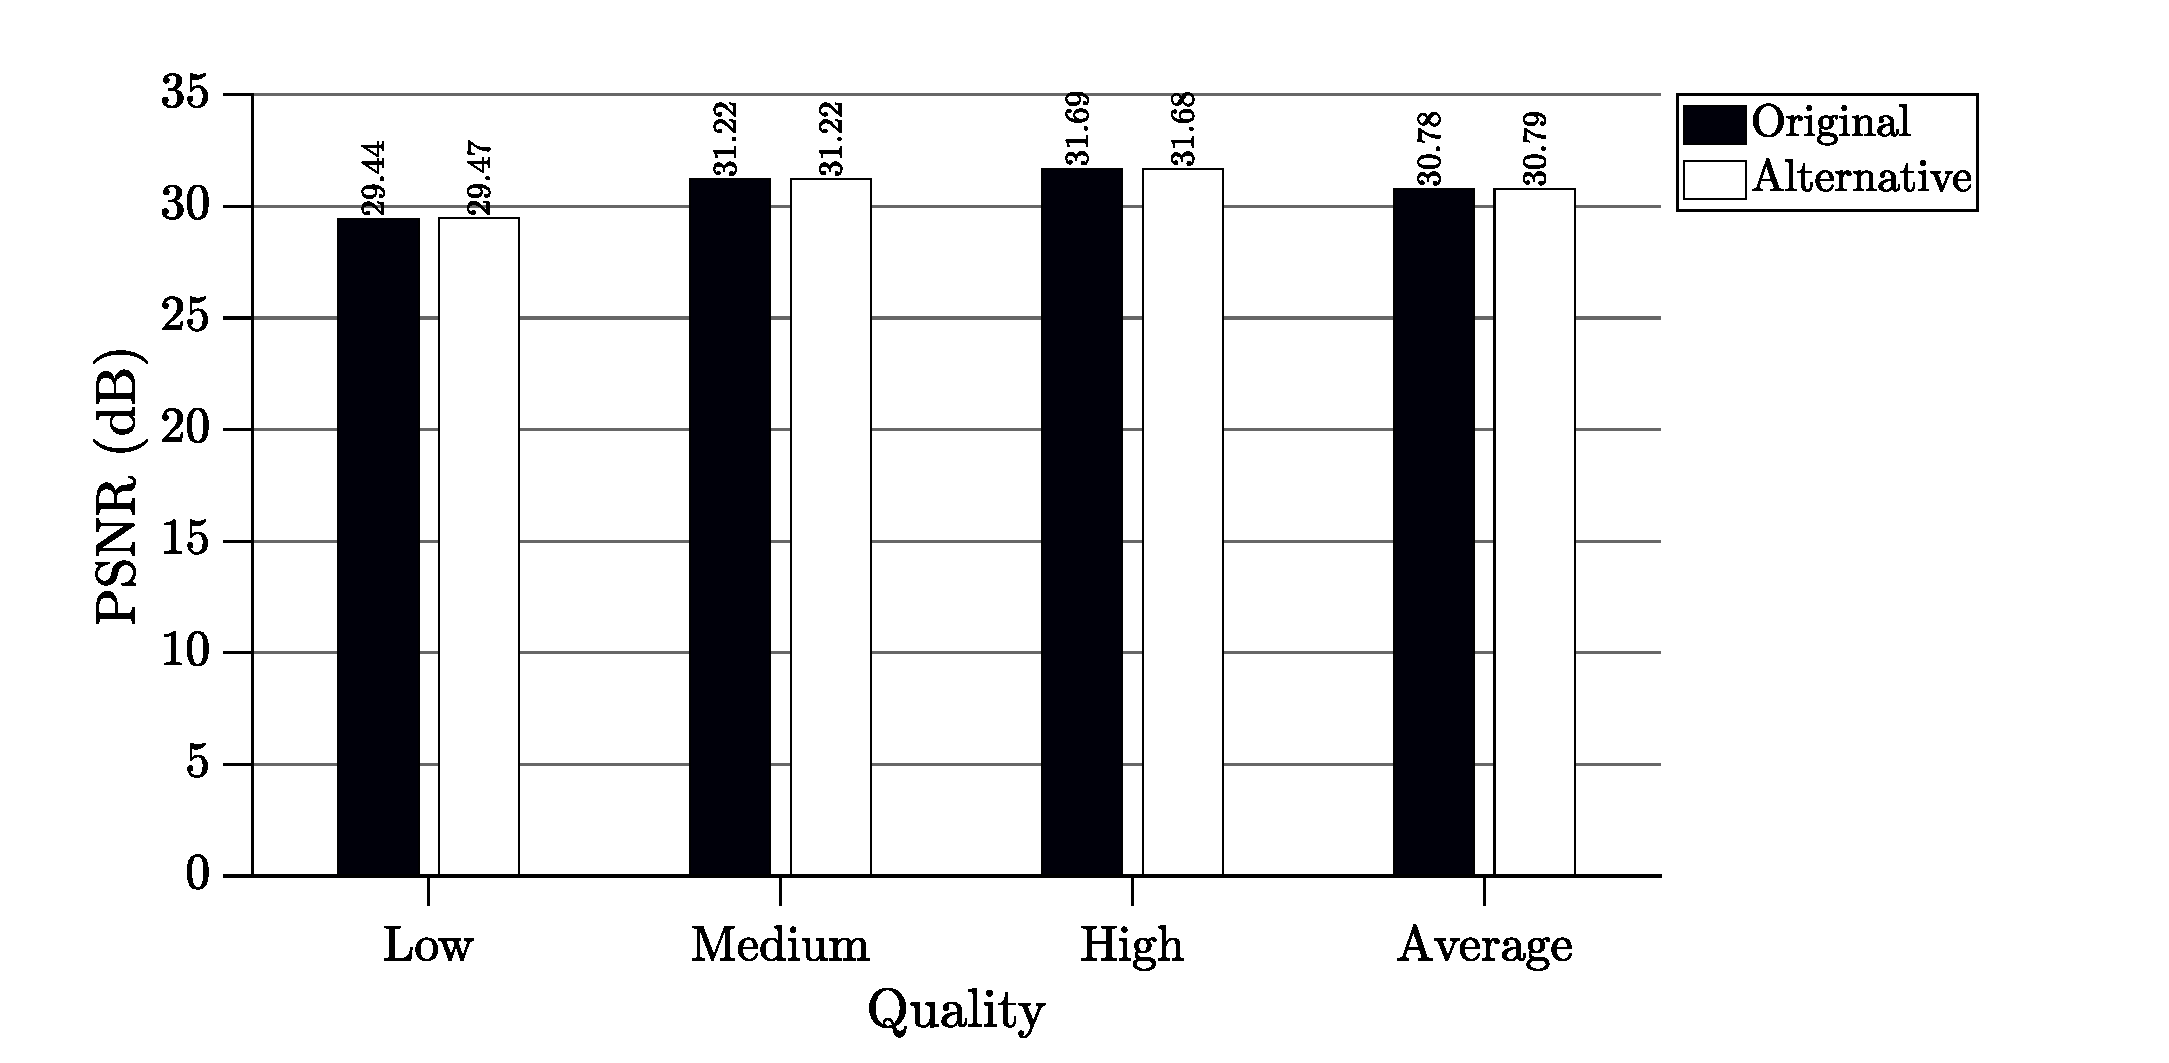
\includegraphics[width=\textwidth]{Sections/4DevelopedArchitecture/Figures/buttmultqual.eps}
    \caption{Obtained quality with original vs alternative \emph{DCT} implementation.}
    \label{fig:buttqual}
\end{figure}

\begin{figure}[!htpb]
    \centering
    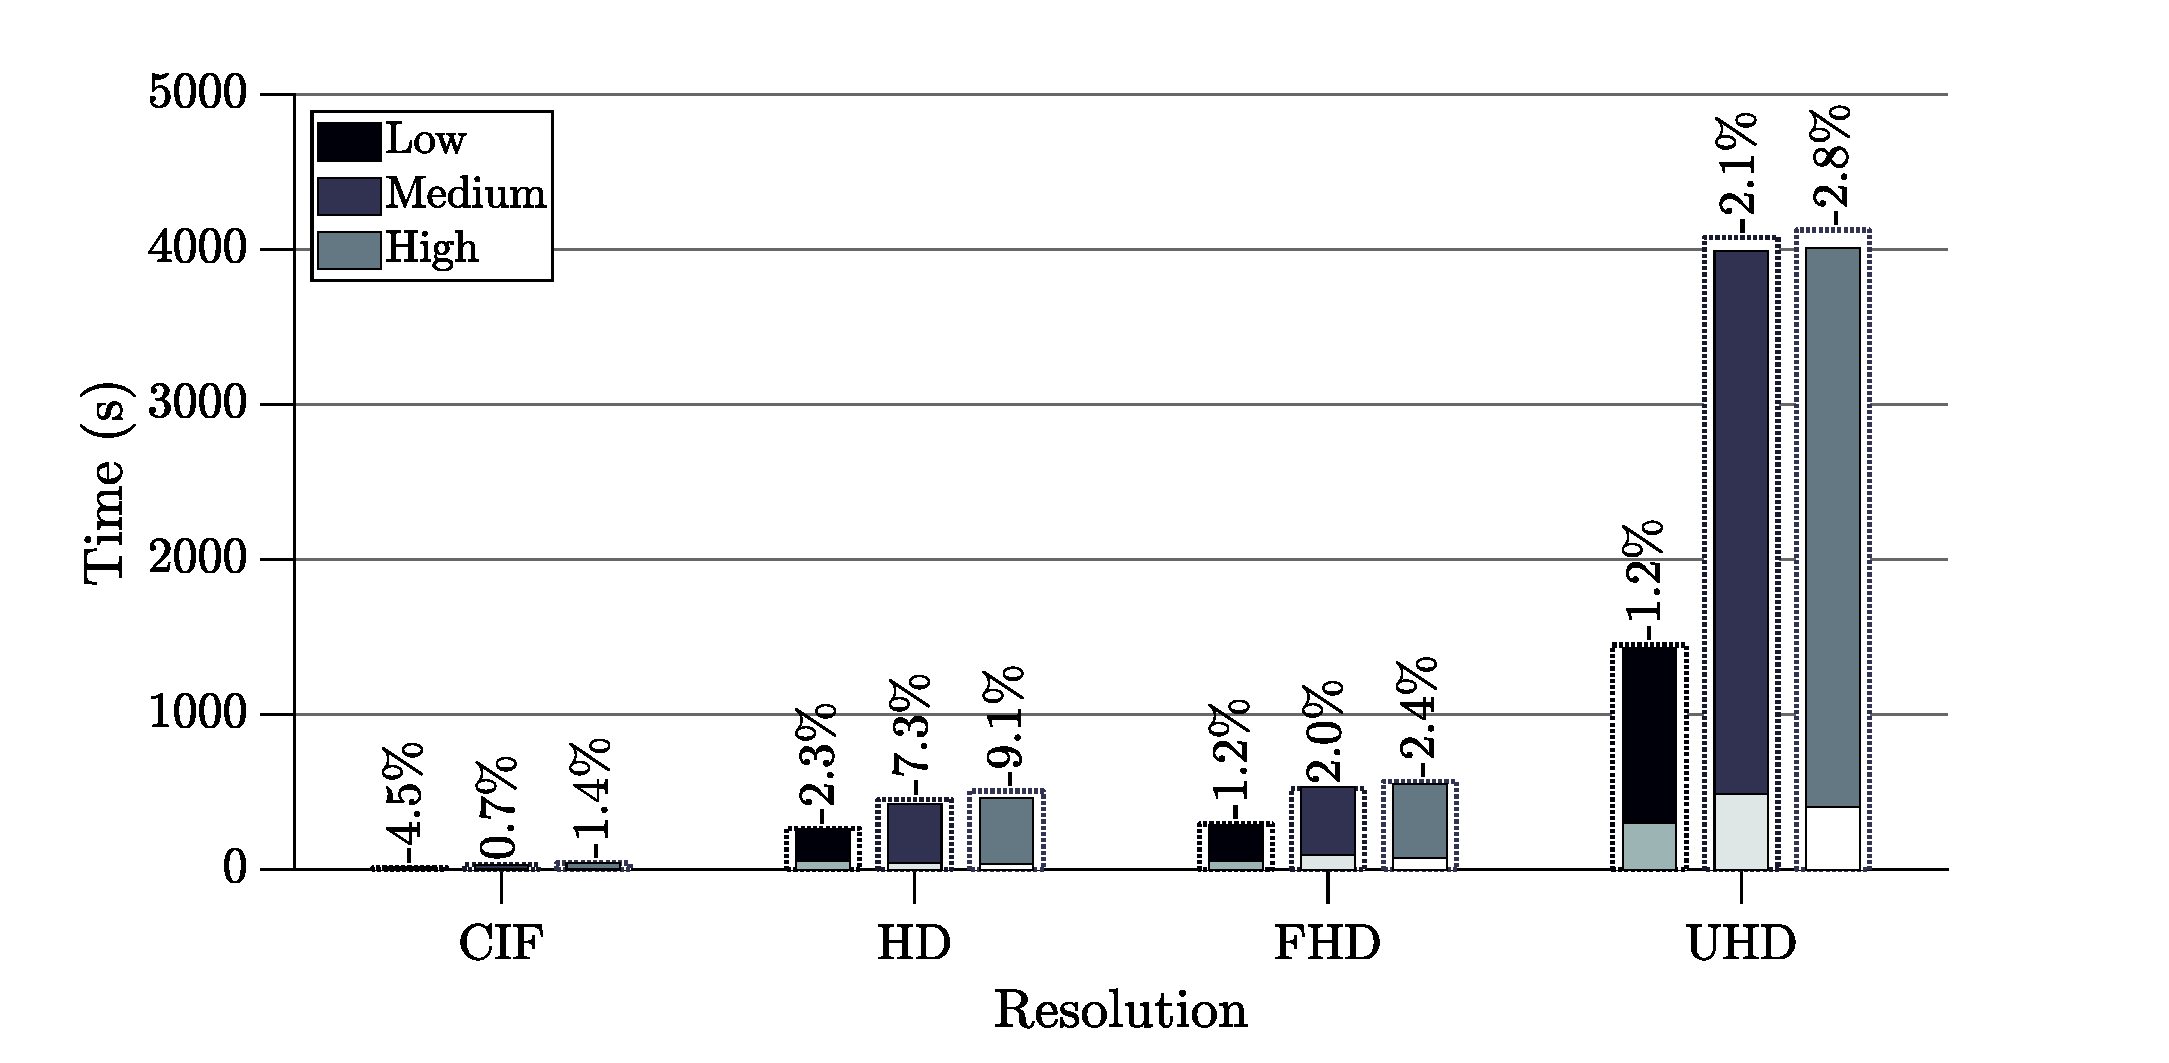
\includegraphics[width=\textwidth]{Sections/4DevelopedArchitecture/Figures/buttmulttime.eps}
    \caption{Encoding time with original vs alternative \emph{DCT} implementation.}
    \label{fig:butttime}
\end{figure}

As shown, with the performed changes, the encoding time was, in average, reduced by $2.9\%$ for all quality objectives, while maintaining the output PSNR, making this a suitable \emph{DCT} implementation for an \emph{AV1} encoder. Although the performance improvement is rather diminishing once considered the full encoding cycle, it is a step toward a possible realtime encoding implementation.

These results allow to advance to a hardware implementation, since the obtained architecture can heavily benefit from parallelization and, due to the discard of the \texttt{cospi} array, would need less memory than the original architecture.

%%%%%%%%%%%%%%%%%%%%%%%%%%%%%%%%%%%%%%%%%%%%%%%%%%%%%%%%%%%%%%%%%%%%%%%%%%%%%%
\section{Hardware Implementations}

On the subject of hardware prototyping, \glspl{fpga} have gained massive popularity within developers, both due to its applicability, as well as ease of use. Additionally, in recent years, there have been major developments in software platforms that allow for the synthesis of FPGA designs as \glspl{asic}, such as \emph{Cadence}'s \emph{Genus} or \emph{Synopsys' Design Compiler} \cite{GenusSynthesisSolution, DesignCompilerGraphical}. 

This way, the chosen platform for the development of the hardware architectures was \emph{Xilinx}'s \emph{Vivado}, due to the wide availability of its FPGAs, as well as for the wide support from its community. The designs and test benches were described in \gls{vhdl}.

With an efficient algorithm for each of the supported vector sizes, the first objective was to develop a hardware architecture to implement each of the 1D \emph{DCT}s individually, and group them on a single block at a later stage. Two different architectures were developed. The first implements each of the \emph{DCT} blocks individually, while the latter uses sub-blocks of each \emph{DCT}, in order to achieve the final result. These architectures are explained in the following Sections.

With this approach, it was hopped to reach an architecture that englobed all the \emph{DCT} kernels, allowing to easily chose between each of them, depending on the desired choices made in the beginning of the transform stage.

%%%%%%%%%%%%%%%%%%%%%%%%%%%%%%%%%%%%%%%
\subsection{\emph{Individual 1D DCT} Hardware Design}

The hardware implementations followed the same scheme as the corresponding software counterparts. By this it is meant that the flow of the input towards the output is done in individual and sequential stages. The main difference between these implementations is that in hardware, all of the intermediary signals within each stage are calculated in parallel. 

However, in order to achieve an efficient hardware implementation, some additional measures must be taken into account, mainly when considering the multiplication of signals by the cosine coefficients and re-scaling.

Consider an hypothetical operation performed in the software version, where two intermediary signals, \texttt{x1} and \texttt{x2}, get multiplied by some constant, added, and finally rescaled. In $C$, this operation is easily described in a single line of code, as shown in Figure \ref{fig:hardsoft}. However, to perform the same operation on an hardware descriptive language, some additional steps must be taken. The seemingly simple operation done in software must be deconstructed in various sequential steps, controlled by a clock signal. The operation shown in this Figure is repeated throughout the various \emph{DCT} implementations in hardware, making it the key to the development of the parallel architectures.

\begin{figure}[!htbp]
    \centering
    \begin{tikzpicture}[%
    >={Triangle[length=6pt,angle'=28]},
    start chain=going below,    % General flow is left-to-right
    node distance=5mm and 16mm, % Global setup of box spacing
    every join/.style={norm},   % Default linetype for connecting boxes
    scale=0.7, every node/.style={transform shape},
    ]

    \tikzset{
    base/.style={draw, on chain, on grid, align=center, minimum height=3.5ex},
    proc/.style={base, rectangle, fill=black!10},
    inout/.style={base,trapezium,trapezium left angle=70,trapezium right angle=-70, fill=black!12},
    term/.style={proc, rounded corners},
    sum/.style={base, circle, inner sep=0pt, radius=0.4cm, fill=black!8},
    % coord node style is used for placing corners of connecting lines
    coord/.style={coordinate, on chain, on grid, node distance=6mm and 40mm},
    % nmark node style is used for coordinate debugging marks% -------------------------------------------------
    % Connector line styles for different parts of the diagram
    norm/.style={ar, draw},
    free/.style={ar, draw, green3},
    cong/.style={ar, draw, red3},
    it/.style={font={\small\itshape}},
    ar/.style={->, line width=0.4mm},
    nar/.style={ar, red!75!black},
    pathcos/.style={font=\small, sloped}
    }

    \begin{scope}        
        \node [inout] (x1) {\texttt{x1}};
        \node [sum, right=of x1, join] (s1) {$\mathbf{\times}$};
        \node [proc, above=1cm of s1] (a) {\texttt{a}};
            \draw[ar] (a) -- (s1);

        \node [inout, below=1cm of x1] (x2) {\texttt{x2}};      
        \node [sum, right=of x2, join] (s2) {$\mathbf{\times}$};
        \node [below=1cm of s2, proc] (b) {\texttt{b}};
            \draw[ar] (b) -- (s2);

        \node [below left=3.5cm and 1cm of x2, align=center, font={\bfseries}] (clk) {Sinal de\\Relógio};
            \draw[thick] ($(clk.east)+(0.5,0)$) -- (x2 |- clk.east) -- ++(0,0.5) coordinate (inReg) -- ++(0.8,0) -- ++(0,-0.5) -- ++(0.8,0) -- ++(0,0.5) coordinate (mult) -- ++(0.8,0) -- ++(0,-0.5) -- ++(0.8,0) -- ++(0,0.5) coordinate (sum) -- ++(0.8,0) -- ++(0,-0.5) -- ++(0.8,0) -- ++(0,0.5) coordinate (shift) -- ++(0.8,0) -- ++(0,-0.5) -- ++(0.8,0) -- ++(0,0.5) coordinate (out) -- ++(0.8,0);
        
        \node[align=center,anchor=north, font={\bfseries\small}, yshift=21mm, draw=darkgray, thin] (lab1) at (mult) {Multiplicação};
            \draw[dashed] (mult) --(lab1);
        \node[align=center,anchor=north, font={\bfseries\small}, yshift=12mm, draw=darkgray, thin] (lab2) at (sum) {Soma};
            \draw[dashed] (sum) --(lab2);
        \node[align=center,anchor=north, font={\bfseries\small}, yshift=7mm, draw=darkgray, thin] (lab3) at (shift) {Shift};
            \draw[dashed] (shift) --(lab3);

        \path (s1) -- (s2) node[midway, rotate=90] (mid_s) {};
        \node [sum, right=of mid_s] (s3) {$\mathbf{+}$};
            \draw[ar] (s1.east) -- (s3);
            \draw[ar] (s2.east) -- (s3);

        \node[draw, fill=black!10, right=16mm of s3.center, anchor=center] (sh8) {\texttt{>>8}};
            \draw[ar] (s3) -- (sh8);

        \node[inout, right=of sh8, anchor=center] (y) {\texttt{y}};
            \draw[ar] (sh8) -- (y);

        \path (x1) -- (x2) node[midway, rotate=90] (mid_x) {};
        \path (mid_x) -- (y) node[midway, rotate=90] (center) {};        
        \node[above=3cm of center] (eq) {\texttt{y = (a*x1 + b*x2)>>8;}};        
    \end{scope}

    \begin{pgfonlayer}{background}
        \path (clk.west |- a.north)+(-5mm,2mm) node (a11) {};
        \path (y.east |- clk.south)+(20mm,-2mm) node (a21) {};
        \path[fill=black!2,rounded corners, draw=black!50, dashed]
          (a11) rectangle (a21);
        \path (y.east |- a.north)+(20mm,2mm) node (a22) {};
            \path (a21) -- (a22) node[midway, rotate=90, yshift=0.5cm] (mid_right) {\textbf{Hardware}};

        \path (clk.west |- eq.north)+(-5mm,7mm) node (a11) {};
        \path (y.east |- eq.south)+(20mm,-7mm) node (a21) {};
        \path[fill=black!2,rounded corners, draw=black!50, dashed]
          (a11) rectangle (a21);
        \path (y.east |- eq.north)+(20mm,7mm) node (a22) {};
            \path (a21) -- (a22) node[midway, rotate=90, yshift=0.5cm] (mid_right) {\textbf{Software}};
    \end{pgfonlayer}
\end{tikzpicture}
    \caption{Comparison between software and hardware implementation of multiplication, sum and re-scaling}
    \label{fig:hardsoft}
\end{figure}

Due to advances in \emph{VHDL} compilers and supporting libraries, both multiplication, shifts and additions are easily described, on a similar manner to a higher level language. Although on previous generations there would be some added benefits of implementing a multiplication by shifting and adding an input, as shown in Equation \ref{eq:multshift}, the improvements done in most recent years allow for similar architectures to be implemented, with less effort.

\begin{equation} \label{eq:multshift}
    \texttt{15 * x1} \equiv \texttt{(x1<<3) + (x1<<2) + (x1<<1) + x1}
\end{equation}

Taking these measures into consideration, the development of the 1D transforms becomes similar to all vector sizes. The software implementations are composed of alternating stages of simple summing operations, with more complex multiplying, sum and shift cycles. Therefore, the hardware counterparts are composed of three different blocks:

\begin{itemize}
    \item \emph{Summing Stages} where the inputs get added according to the previously shown butterfly schemes;
    \item \emph{Multiplier Stages}, which multiply the necessary inputs by the corresponding cosine coefficients;
    \item \emph{Shift Stages} that rescale the coefficients.
\end{itemize} 

Although these blocks are unique between transform sizes, and even within the same \emph{DCT}, the operations performed within are similar between all the vector sizes.

In order to ensure the correct pipelining of the \emph{Transform} process, each stage is controlled by an \emph{enable} flag, \texttt{en}, which signals the start of the block's process. Once it is concluded, the block outputs an indicator, \texttt{valOut}, that acts as the enable for the following stage, creating a daisy chain of stages. The last stage's \texttt{valOut} acts as the indication of the conclusion of the \emph{Transform} operation.

All blocks are controlled by the same \emph{clock} and \emph{reset} signals. The first triggers the internal processes on its ascending flank. The latter signals all internal registers to be put to 0 (its initial stage).

A simplified version of \emph{DCT4}'s hardware implementation is represented in Figure \ref{fig:harddct4v1}. In here, the direction of the arrow represents if the corresponding signal is a \emph{input} or \emph{output}. The numbering of the output coefficients is done accordingly to the software implementation.

\begin{figure}[!htbp]
    \centering
    \begin{tikzpicture}[%
    >={Triangle[length=6pt,angle'=28]},
    start chain=going below,    % General flow is left-to-right
    node distance=5mm and 20mm, % Global setup of box spacing
    every join/.style={norm},   % Default linetype for connecting boxes
    ]

\tikzset{
  base/.style={draw, on chain, on grid, align=center, minimum height=3.5ex},
  reg/.style={base, rectangle, minimum width=2.5em, minimum height=2em,fill=black!15},
  proc/.style={base, rectangle, minimum width=4em, minimum height=8em, fill=black!15},
  inout/.style={base,trapezium,trapezium left angle=70,trapezium right angle=-70, fill=blue!12},
  term/.style={proc, rounded corners},
  sum/.style={base, circle, inner sep=0pt, radius=0.4cm, fill=black!15},
  % coord node style is used for placing corners of connecting lines
  coord/.style={coordinate, on chain, on grid, node distance=6mm and 40mm},
  % nmark node style is used for coordinate debugging marks% -------------------------------------------------
  % Connector line styles for different parts of the diagram
  norm/.style={aar, draw},
  free/.style={aar, draw, green3},
  cong/.style={aar, draw, red3},
  it/.style={font={\small\itshape}},
  nar/.style={aar, red!75!black},
  aar/.style={->, line width=0.4mm},
  pathcos/.style={font=\small, sloped}
}    

\begin{scope}


\end{scope}
\end{tikzpicture}
    \caption{1D \emph{DCT 4} hardware implementation}
    \label{fig:harddct4v1}
\end{figure}

All data signals and corresponding internal registers are represented with 32 bits. Although this increases the necessary footprint, this measure simplifies the development and integration between different transforms. Nonetheless, some additional measures were taken in the hardware description files, in order to easily change the number of used bits (\emph{\gls{genmap}}), at a later stage.

As a final measure to simplify the development process, the \emph{kernels} are implemented using the smaller sizes as a constituting block. As shown in \cite{wen-hsiungchenFastComputationalAlgorithm1977}, all transform sizes greater than $4$ englobe the same sequence of operations as the smaller counterparts, on one subset of its intermediary coefficients. This way, each of the smaller \emph{1D-DCT} blocks may be inserted into the size immediately above it.

As an example, \emph{DCT8}'s hardware implementation is represented in Figure \ref{fig:harddct8v1}. There, it is observable that the architecture is similarly composed of the same blocks as the previous implementation. However, after the first summing stage, the first four intermediary coefficients are input into \emph{DCT4}. 

\begin{figure}[!htbp]
    \centering
    \begin{tikzpicture}[%
    >={Triangle[length=6pt,angle'=28]},
    start chain=going below ,    % General flow is left-to-right
    node distance=5mm and 20mm, % Global setup of box spacing
    every join/.style={norm},   % Default linetype for connecting boxes
    scale=0.8, 
    every node/.style={transform shape},
    circuit logic US, every circuit symbol/.style={thick}
    ]

  \tikzset{
    base/.style={draw, on chain, on grid, align=center, minimum height=3.5ex},
    reg/.style={base, rectangle, minimum width=2.5em, minimum height=2em,fill=black!15},
    proc/.style={base, rectangle, minimum width=4em, minimum height=8em, fill=black!15},
    inout/.style={base,trapezium,trapezium left angle=70,trapezium right angle=-70, fill=blue!12},
    term/.style={proc, rounded corners},
    sum/.style={base, circle, inner sep=0pt, radius=0.4cm, fill=black!15},
    % coord node style is used for placing corners of connecting lines
    coord/.style={coordinate, on chain, on grid, node distance=6mm and 40mm},
    % nmark node style is used for coordinate debugging marks% -------------------------------------------------
    % Connector line styles for different parts of the diagram
    norm/.style={ar32, draw},
    free/.style={ar32, draw, green3},
    cong/.style={ar32, draw, red3},
    it/.style={font={\small\itshape}},
    nar/.style={ar32, red!75!black},
    ar32/.style={->, line width=0.8mm},   
    b32/.style={line width=0.8mm},    
    ar1/.style={->, line width=0.4mm}
  }    

  \begin{scope}[y=-1cm]
    \begin{scope}
      %\draw[step=1cm, very thin, lightgray] (0,0) grid (14,30);
      
      %% Inputs
      \draw [black,very thick] (1,4) circle (1mm) node [right, rotate=90, xshift=1mm] {\texttt{Clock}};
        \draw [ar1] (1,4.1) |- (9.5,16);
        \draw [ar1] (1,4.1) |- (4,10.5);
        \draw [ar1] (1,4.1) -- (1,8.6) -- ++(7.7,0) |- (9.5,11.5-1);
        \draw [ar1] (1,4.1) |- (4,7.5-1);
        %\draw [ar32] (1,4.1) |- (4,3.5-1);
      \draw [black,very thick] (2,4) circle (1mm) node [right, rotate=90, xshift=1mm] {\texttt{Reset}};
        \draw [ar1] (2,4.1) |- (9.5,15.5);
        \draw [ar1] (2,4.1) |- (4,10);
        \draw [ar1] (2,4.1) -- (2,8.4) -- ++(6.9,0) |- (9.5,11-1);
        \draw [ar1] (2,4.1) |- (4,7.5-1);
        %\draw [ar32] (2,4.1) |- (4,3.5-1);
      \draw [black,very thick] (3,4) circle (1mm) node [right, rotate=90, xshift=1mm] {\texttt{Enable}};
        \draw [ar1] (3,4.1) |- (4,5.5);
      \foreach \x in {0,...,3}
        \draw [black,very thick] (5+\x,4) circle (1mm) node [right, rotate=90, xshift=1mm] (dIn\x) {\texttt{dataIn\x}};
      \foreach \x in {4,...,7}
        \draw [black,very thick] (6+\x,4) circle (1mm) node [right, rotate=90, xshift=1mm] (dIn\x) {\texttt{dataIn\x}};

      %% In Register
      %\node (inReg) at (5-1,2-1) [draw,thick,minimum width=10cm,minimum height=3cm, rounded corners, anchor=north west, fill=black!8, font={\large}] {\textbf{Input Register}};
      %\node (enInReg) at (5-1,2.5-1) [right, font={\small}] {\texttt{en}};
      %\node (resInReg) at (5-1,3-1) [right, font={\small}] {\texttt{res}};
      %\node (clkInReg) at (5-1,3.5-1) [right, font={\small}] {\texttt{clk}};
      %\node (valoutInReg) at (5-1,4.5-1) [right, font={\small}] {\texttt{valOut}};
      %  \draw [ar32] (5-1,4.5-1) -- ++(-1,0) |- (5-1,6.5-1);

      %% Stage 1 Sum
      \node (St1) at (5-1,6-1) [draw,thick,minimum width=10cm,minimum height=3cm, rounded corners, anchor=north west, fill=black!8, font={\large}] {\textbf{Stage 1: Sum}};
      \node (enSt1) at (5-1,6.5-1) [right, font={\small}] {\texttt{en}};
      \node (resSt1) at (5-1,7-1) [right, font={\small}] {\texttt{res}};
      \node (clkSt1) at (5-1,7.5-1) [right, font={\small}] {\texttt{clk}};
      \node (valoutSt1) at (5-1,8.5-1) [right, font={\small}] {\texttt{valOut}};
        \draw [ar1] (5-1,8.5-1) -- ++(-1,0) |- (5-1,10.5-1);
        \draw [ar1] (5-1,8.5-1) -- ++(-1,0) -- ++(0,0.7) -- ++(6.1,0) |- (9.5,10.5-1);

      %% DCT4
      \node (DCT4) at (4,9) [draw,thick,minimum width=4.5cm,minimum height=3cm, rounded corners, anchor=north west, fill=black!12, font={\large\bfseries}, align=center] {DCT4};
      \node (enSt2M) at (5-1,10.5-1) [right, font={\small}] {\texttt{en}};
      \node (resSt2M) at (5-1,11-1) [right, font={\small}] {\texttt{res}};
      \node (clkSt2M) at (5-1,11.5-1) [right, font={\small}] {\texttt{clk}};
      \node (valoutDCT4) at (5-1,12.5-1) [right, font={\small}] {\texttt{valOut}};
    
      %% Stage 2 Mult
      \node (St2M) at (9.5,9) [draw,thick,minimum width=4.5cm,minimum height=3cm, rounded corners, anchor=north west, fill=black!8, font={\large\bfseries}, align=center] {Stage 2:\\Multiplier};
      \node (enSt2M) at (9.5,10.5-1) [right, font={\small}] {\texttt{en}};
      \node (resSt2M) at (9.5,11-1) [right, font={\small}] {\texttt{res}};
      \node (clkSt2M) at (9.5,11.5-1) [right, font={\small}] {\texttt{clk}};
      \node (valoutSt2M) at (9.5,12.5-1) [right, font={\small}] {\texttt{valOut}};
        \draw [ar1] (9.5,12.5-1) -- ++(-0.5,0) -- ++(0,1.5) coordinate (etc);
    
      \foreach \x in {0,...,4}
        \node at (etc) [left, rotate=90, xshift=-1mm, yshift=-\x cm, font={\bfseries}] {...};

      %% Stage 4 Shift
      \foreach \x in {0,...,3}
        \draw [ar32] (10+\x,14) -- ++(0,0.5);
      \draw [ar1] (9,14) |- (9.5,15);
      \node (St4S) at (9.5,14.5) [draw,thick,minimum width=4.5cm,minimum height=3cm, rounded corners, anchor=north west, fill=black!8, font={\large\bfseries}, align=center] {Stage 4:\\Shift};
      \node (enSt2S) at (9.5,15) [right, font={\small}] {\texttt{en}};
      \node (resSt2S) at (9.5,15.5) [right, font={\small}] {\texttt{res}};
      \node (clkSt2S) at (9.5,16) [right, font={\small}] {\texttt{clk}};
      \node (valoutSt2S) at (9.5,17) [right, font={\small}] {\texttt{valOut}}; 
        %\draw [ar32] (9.5,20.5-1) -| (2-1,20.5); 
        
        \node[and gate,inputs={nnnn}, point down] (and1) at (1,18)    {};
            \draw[ar1] (valoutSt2S) -| (and1.input 1);
            \draw[ar1] (valoutDCT4) -| (and1.input 4);
            \draw[ar1] (and1.output) -- (1, 19.5);
            \draw[line width=0.4mm] (1, 19.5) -- ++(0, 0.4);

      %% Outputs
      \draw [black,very thick] (2-1,20) circle (1mm) node [left, rotate=90, xshift=-1mm] {\texttt{validOut}};
      \draw [black,very thick] (5+0,20) circle (1mm) node [left, rotate=90, xshift=-1mm] (dOut0) {\texttt{dataOut0}};
      \draw [black,very thick] (5+1,20) circle (1mm) node [left, rotate=90, xshift=-1mm] (dOut4) {\texttt{dataOut4}};
      \draw [black,very thick] (5+2,20) circle (1mm) node [left, rotate=90, xshift=-1mm] (dOut2) {\texttt{dataOut2}};
      \draw [black,very thick] (5+3,20) circle (1mm) node [left, rotate=90, xshift=-1mm] (dOut6) {\texttt{dataOut6}};
      
      \draw [black,very thick] (6+4,20) circle (1mm) node [left, rotate=90, xshift=-1mm] (dOut1) {\texttt{dataOut1}};
      \draw [black,very thick] (6+5,20) circle (1mm) node [left, rotate=90, xshift=-1mm] (dOut5) {\texttt{dataOut5}};
      \draw [black,very thick] (6+6,20) circle (1mm) node [left, rotate=90, xshift=-1mm] (dOut3) {\texttt{dataOut3}};
      \draw [black,very thick] (6+7,20) circle (1mm) node [left, rotate=90, xshift=-1mm] (dOut7) {\texttt{dataOut7}};

      \foreach \x in {0,...,3} {
        %\draw[ar32] (5+\x,-1mm) -- ++(0, -0.9cm);
        \draw[ar32] (5+\x,4.1) -- ++(0, -0.9cm);
        \draw[ar32] (5+\x,8) -- ++(0, -1cm);
        \draw[ar32] (5+\x,12) -- ++(0, -7.5cm);       
        \draw[b32] (5+\x,19.5) -- ++(0, -0.4cm);
      }
      \foreach \x in {4,...,7} {
        %\draw[ar32] (6+\x,-1mm) -- ++(0, -0.9cm);
        \draw[ar32] (6+\x,4.1) -- ++(0, -0.9cm);
        \draw[ar32] (6+\x,8) -- ++(0, -1cm);
        \draw[ar32] (6+\x,12) -- ++(0, -1cm);
        \draw[ar32] (6+\x,17.5) -- ++(0, -2cm);
        \draw[b32] (6+\x,19.5) -- ++(0, -0.4cm);
      }
    \end{scope}
    \begin{pgfonlayer}{background}
      % Left-top corner of the background rectangle
      \node (a11) at (0,4.5) {};
      % Right-bottom corner of the background rectanle
      \node (a21) at (14.5,19.5) {};
      % Draw the background
      \path[fill=black!3,rounded corners, draw, very thick]
        (a11) rectangle (a21);
      \node (a31) at (1.5,19.5) {};
      \path (a11) -- (a31) node[midway, rotate=90, yshift=1.3cm, font={\huge}] (mid_right) {\textbf{DCT8}};
    \end{pgfonlayer}
  \end{scope}
\end{tikzpicture}
    \caption{Simplified 1D \emph{DCT 8} hardware implementation, with inclusion of \emph{DCT 4}}
    \label{fig:harddct8v1}
\end{figure}

In the same manner, \emph{DCT16} includes \emph{DCT8}, which, as shown, also includes the four input version. This approach causes the smaller blocks to be repeated throughout the various larger architectures, making this approach highly inefficient from the chip's utilization standpoint.

Nonetheless, in order to draw conclusions as to the correct functioning of the internal stages, as well as to see possible gains from the following implementations, the architecture from Figure \ref{fig:fullv1} was developed.

\begin{figure}[!htbp]
    \centering
    \begin{tikzpicture}[%
    >={Triangle[length=6pt,angle'=28]},
    start chain=going below ,    % General flow is left-to-right
    node distance=5mm and 20mm, % Global setup of box spacing
    every join/.style={norm},   % Default linetype for connecting boxes
    scale=0.8, 
    every node/.style={transform shape},
    circuit logic US, every circuit symbol/.style={thick}
    ]

  \tikzset{
    base/.style={draw, on chain, on grid, align=center, minimum height=3.5ex},
    reg/.style={base, rectangle, minimum width=2.5em, minimum height=2em,fill=black!15},
    proc/.style={base, rectangle, minimum width=4em, minimum height=8em, fill=black!15},
    inout/.style={base,trapezium,trapezium left angle=70,trapezium right angle=-70, fill=blue!12},
    term/.style={proc, rounded corners},
    sum/.style={base, circle, inner sep=0pt, radius=0.4cm, fill=black!15},
    % coord node style is used for placing corners of connecting lines
    coord/.style={coordinate, on chain, on grid, node distance=6mm and 40mm},
    % nmark node style is used for coordinate debugging marks% -------------------------------------------------
    % Connector line styles for different parts of the diagram
    norm/.style={aar, draw},
    ar32/.style={->, line width=0.8mm},   
    b32/.style={line width=0.8mm},    
    ar1/.style={->, line width=0.4mm}  
  }    

  \begin{scope}[y=-1cm]
    \begin{scope}
      %\draw[step=1cm, very thin, lightgray] (0,0) grid (14,20);            
        
        %% Inputs/Outputs

        % IN/OUT 0-3
        \foreach \x in {0,...,3}
            \draw [black,very thick] (0,1+0.5*\x) circle (1mm) node [left, xshift=-1mm] (dIn\x) {\texttt{dataIn\x}};      
        \node at (0,3) [anchor=east, rotate=90, font={\bfseries}] {...};
            
            \foreach \x in {0,...,3} {
                \draw[ar32] (0.1,1+0.5*\x) -- ++(1.9,0);                
            }
            \draw[ar32] (1,1) |- (2,4.5);
                \node at (1.5,5) [anchor=east, rotate=90, font={\bfseries}] {...};
            \draw[ar32] (1,4.5) |- (2,8);
                \node at (1.5,8.5) [anchor=east, rotate=90, font={\bfseries}] {...};
            \draw[ar32] (1,8) |- (2,11.5);
                \node at (1.5,12) [anchor=east, rotate=90, font={\bfseries}] {...};
            \draw[ar32] (1,11.5) |- (2,15);
                \node at (1.5,15.5) [anchor=east, rotate=90, font={\bfseries}] {...};

            \draw[ar32] (6.5,1) node [above, font={\small\ttfamily}, align=center, xshift=0.75cm] {DCT4o0} -- ++(1.5,0);
            \node at (7,1) [anchor=east, rotate=90, font={\bfseries}] {...};
            \draw[ar32] (6.5,2) node [above, font={\small\ttfamily}, align=center, xshift=0.75cm] {DCT4o3} -- ++(1.5,0);
            \draw[ar1] (6.5,2.5) node [above, font={\small\ttfamily}, align=center, xshift=0.75cm] {DCT4vo} -- ++(1.5,0);


        % IN 7/DCT8
        \draw [black,very thick] (0,6) circle (1mm) node [left, xshift=-1mm] (dIn7) {\texttt{dataIn7}};      
            \node at (0.25,6.5) [anchor=east, rotate=90, font={\bfseries}] {...};

                \draw[ar32] (0.1,6) -- ++(1.9,0);
                \draw[ar32] (0.5,6) -- ++(0,0.5);

                \draw[ar32] (6.5,4.5) node [above, font={\small\ttfamily}, align=center, xshift=0.75cm] {DCT8o0} -- ++(1.5,0);
                \node at (7,4.5) [anchor=east, rotate=90, font={\bfseries}] {...};
                \draw[ar32] (6.5,5.5) node [above, font={\small\ttfamily}, align=center, xshift=0.75cm] {DCT8o7} -- ++(1.5,0);
                \draw[ar1] (6.5,6) node [above, font={\small\ttfamily}, align=center, xshift=0.75cm] {DCT8vo} -- ++(1.5,0);

        % IN 15/DCT16
        \draw [black,very thick] (0,9.5) circle (1mm) node [left, xshift=-1mm] (dIn15) {\texttt{dataIn15}};      
            \node at (0.25,10) [anchor=east, rotate=90, font={\bfseries}] {...};

                \draw[ar32] (0.1,9.5) -- ++(1.9,0);
                \draw[ar32] (0.5,9.5) -- ++(0,0.5);

                \draw[ar32] (6.5,8) node [above, font={\small\ttfamily}, align=center, xshift=0.75cm] {DCT16o0} -- ++(1.5,0);
                \node at (7,8) [anchor=east, rotate=90, font={\bfseries}] {...};
                \draw[ar32] (6.5,9) node [above, font={\small\ttfamily}, align=center, xshift=0.75cm] {DCT16o15} -- ++(1.5,0);
                \draw[ar1] (6.5,9.5) node [above, font={\small\ttfamily}, align=center, xshift=0.75cm] {DCT16vo} -- ++(1.5,0);

        % IN 31/DCT32
        \draw [black,very thick] (0,13) circle (1mm) node [left, xshift=-1mm] (dIn31) {\texttt{dataIn31}};      
            \node at (0.25,13.5) [anchor=east, rotate=90, font={\bfseries}] {...};

                \draw[ar32] (0.1,13) -- ++(1.9,0);
                \draw[ar32] (0.5,13) -- ++(0,0.5);

                \draw[ar32] (6.5,11.5) node [above, font={\small\ttfamily}, align=center, xshift=0.75cm] {DCT32o0} -- ++(1.5,0);
                \node at (7,11.5) [anchor=east, rotate=90, font={\bfseries}] {...};
                \draw[ar32] (6.5,12.5) node [above, font={\small\ttfamily}, align=center, xshift=0.75cm] {DCT32o31} -- ++(1.5,0);
                \draw[ar1] (6.5,13) node [above, font={\small\ttfamily}, align=center, xshift=0.75cm] {DCT32vo} -- ++(1.5,0);

        % IN 63/DCT64
        \draw [black,very thick] (0,16.5) circle (1mm) node [left, xshift=-1mm] (dIn63) {\texttt{dataIn63}};      

                \draw[ar32] (0.1,16.5) -- ++(1.9,0);
            
                \draw[ar32] (6.5,15) node [above, font={\small\ttfamily}, align=center, xshift=0.75cm] {DCT64o0} -- ++(1.5,0);
                \node at (7,15) [anchor=east, rotate=90, font={\bfseries}] {...};
                \draw[ar32] (6.5,16) node [above, font={\small\ttfamily}, align=center, xshift=0.75cm] {DCT64o63} -- ++(1.5,0);
                \draw[ar1] (6.5,16.5) node [above, font={\small\ttfamily}, align=center, xshift=0.75cm] {DCT64vo} -- ++(1.5,0);

        % Clock
        \draw [black,very thick] (0,18) circle (1mm) node [left, xshift=-1mm] (clk) {\texttt{Clock}};            
            \draw[ar1] (0.1,18) -- (2.2,18) -- (2.2,3.5) -| (3,3);
            \draw[ar1] (2.2,7) -| (3,6.5);
            \draw[ar1] (2.2,10.5) -| (3,10);
            \draw[ar1] (2.2,14) -| (3,13.5);
            \draw[ar1] (2.2,17.5) -| (3,17);
            \draw[ar1] (2.2,18) -- (8,18);
        
        % Reset
        \draw [black,very thick] (0,18.5) circle (1mm) node [left, xshift=-1mm] (res) {\texttt{Reset}};
            \draw[ar1] (0.1,18.5) -- (2.5,18.5) -- (2.5,3.8) -| (3.5,3);
            \draw[ar1] (2.5,7.3) -| (3.5,6.5);
            \draw[ar1] (2.5,10.8) -| (3.5,10);
            \draw[ar1] (2.5,14.3) -| (3.5,13.5);
            \draw[ar1] (2.5,17.8) -| (3.5,17);
            \draw[ar1] (2.5,18.5) -- (8,18.5);

        % Enable
        \draw [black,very thick] (0,19) circle (1mm) node [left, xshift=-1mm] (enin) {\texttt{Enable}};
            \draw[ar1] (0.1,19) -- (8,19);
            
            \draw[ar1] (8,3.5) node [above, font={\small\ttfamily}, align=center, xshift=-0.75cm] {DCT4En} -| (4,3) ;
            \draw[ar1] (8,7) node [above, font={\small\ttfamily}, align=center, xshift=-0.75cm] {DCT8En} -| (4,6.5);
            \draw[ar1] (8,10.5) node [above, font={\small\ttfamily}, align=center, xshift=-0.75cm] {DCT16En} -| (4,10);
            \draw[ar1] (8,14) node [above, font={\small\ttfamily}, align=center, xshift=-0.75cm] {DCT32En} -| (4,13.5);
            \draw[ar1] (8,17.5) node [above, font={\small\ttfamily}, align=center, xshift=-0.75cm] {DCT64En} -| (4,17);

        % Select
        \draw [black,very thick] (0,19.5) circle (1mm) node [left, xshift=-1mm] (selin) {\texttt{Select}};
            \draw[ar1] (0.1,19.5) -- (8,19.5) node [midway, below, font={\small\ttfamily}] {3};
            \draw[line width=0.4mm] (3.9,19.6) -- (4.1,19.4);

        %% Outputs
        \foreach \x in {0,...,3} {
            \draw [black,very thick] (14,7.5+0.5*\x) circle (1mm) node [right, xshift=1mm] (dout\x) {\texttt{dataOut\x}};      
            \draw [ar32] (12.5,7.5+0.5*\x) -- (13.9,7.5+0.5*\x);      
        }

        \node at (14,10) [anchor=east, rotate=90, font={\bfseries}] {...};
        \foreach \x in {0,...,3} {
            \draw [black,very thick] (14,11.5+0.5*\x) circle (1mm) node [right, xshift=1mm] (dout6\x) {\texttt{dataOut6\x}};      
            \draw [ar32] (12.5,11.5+0.5*\x) -- (13.9,11.5+0.5*\x);      
        }

        \draw [black,very thick] (14,14.5) circle (1mm) node [right, xshift=1mm] (valOut) {\texttt{validOut}};      
            \draw [ar32] (12.5,14.5) -- (13.9,14.5);      


    %% DCT 4
    \node (DCT4) at (2,0.5) [draw,thick,minimum width=4.5cm,minimum height=2.5cm, rounded corners, anchor=north west, fill=black!12, font={\large\bfseries}, align=center] {DCT4};
    \node (enSt2M) at (DCT4.south west) [rotate=90, xshift=1mm, right, font={\small}, yshift=-1cm] {\texttt{clk}};
    \node (resSt2M) at (DCT4.south west) [rotate=90, xshift=1mm, right, font={\small}, yshift=-1.5cm] {\texttt{res}};
    \node (clkSt2M) at (DCT4.south west) [rotate=90, xshift=1mm, right, font={\small}, yshift=-2cm] {\texttt{en}};
    \node (valoutDCT4) at (DCT4.south east) [left, yshift=0.5cm, font={\small}] {\texttt{valOut}};

    %% DCT 8
    \node (DCT8) at (2,4) [draw,thick,minimum width=4.5cm,minimum height=2.5cm, rounded corners, anchor=north west, fill=black!12, font={\large\bfseries}, align=center] {DCT8};
    \node (enSt2M) at (DCT8.south west) [rotate=90, xshift=1mm, right, font={\small}, yshift=-1cm] {\texttt{clk}};
    \node (resSt2M) at (DCT8.south west) [rotate=90, xshift=1mm, right, font={\small}, yshift=-1.5cm] {\texttt{res}};
    \node (clkSt2M) at (DCT8.south west) [rotate=90, xshift=1mm, right, font={\small}, yshift=-2cm] {\texttt{en}};
    \node (valoutDCT8) at (DCT8.south east) [left, yshift=0.5cm, font={\small}] {\texttt{valOut}};

    %% DCT 16
    \node (DCT16) at (2,7.5) [draw,thick,minimum width=4.5cm,minimum height=2.5cm, rounded corners, anchor=north west, fill=black!12, font={\large\bfseries}, align=center] {DCT16};
    \node (enSt2M) at (DCT16.south west) [rotate=90, xshift=1mm, right, font={\small}, yshift=-1cm] {\texttt{clk}};
    \node (resSt2M) at (DCT16.south west) [rotate=90, xshift=1mm, right, font={\small}, yshift=-1.5cm] {\texttt{res}};
    \node (clkSt2M) at (DCT16.south west) [rotate=90, xshift=1mm, right, font={\small}, yshift=-2cm] {\texttt{en}};
    \node (valoutDCT16) at (DCT16.south east) [left, yshift=0.5cm, font={\small}] {\texttt{valOut}};

    %% DCT 32
    \node (DCT32) at (2,11) [draw,thick,minimum width=4.5cm,minimum height=2.5cm, rounded corners, anchor=north west, fill=black!12, font={\large\bfseries}, align=center] {DCT32};
    \node (enSt2M) at (DCT32.south west) [rotate=90, xshift=1mm, right, font={\small}, yshift=-1cm] {\texttt{clk}};
    \node (resSt2M) at (DCT32.south west) [rotate=90, xshift=1mm, right, font={\small}, yshift=-1.5cm] {\texttt{res}};
    \node (clkSt2M) at (DCT32.south west) [rotate=90, xshift=1mm, right, font={\small}, yshift=-2cm] {\texttt{en}};
    \node (valoutDCT32) at (DCT32.south east) [left, yshift=0.5cm, font={\small}] {\texttt{valOut}};

    %% DCT 64
    \node (DCT64) at (2,14.5) [draw,thick,minimum width=4.5cm,minimum height=2.5cm, rounded corners, anchor=north west, fill=black!12, font={\large\bfseries}, align=center] {DCT64};
    \node (enSt2M) at (DCT64.south west) [rotate=90, xshift=1mm, right, font={\small}, yshift=-1cm] {\texttt{clk}};
    \node (resSt2M) at (DCT64.south west) [rotate=90, xshift=1mm, right, font={\small}, yshift=-1.5cm] {\texttt{res}};
    \node (clkSt2M) at (DCT64.south west) [rotate=90, xshift=1mm, right, font={\small}, yshift=-2cm] {\texttt{en}};
    \node (valoutDCT32) at (DCT64.south east) [left, yshift=0.5cm, font={\small}] {\texttt{valOut}};

    %% Select
    \node (sel) at (8,0.5) [draw,thick,minimum width=4.5cm,minimum height=19.5cm, rounded corners, anchor=north west, fill=black!5, font={\large\bfseries}, align=center] {Output's\\Multiplexer};
    \node (selclk) at (sel.south west) [xshift=1mm, yshift=20mm, right, font={\small}] {\texttt{clk}};
    \node (selres) at (sel.south west) [xshift=1mm, yshift=15mm, right, font={\small}] {\texttt{res}};
    \node (selen) at (sel.south west) [xshift=1mm, yshift=10mm, right, font={\small}] {\texttt{en}};
    \node (selin) at (sel.south west) [xshift=1mm, yshift=5mm, right, font={\small}] {\texttt{sel}};



    \end{scope}
    \begin{pgfonlayer}{background}
      
    \end{pgfonlayer}
  \end{scope}
\end{tikzpicture}
    \caption{First version of the complete \emph{DCT} kernel}
    \label{fig:fullv1}
\end{figure}

\clearpage
\printbibliography[heading=subbibliography]
\addcontentsline{toc}{section}{References}